%
%% Section: ARCHITECTURE & DESIGN
%\section{Architecture and Design}
%\label{sec:design}
%
%The option for enabling a community cloud in a community network on which we focus here is to deploy on SNs a cloud management system tailored to community networks. 
%Available popular cloud management platforms, notably
%	OpenStack~\cite{OpenStack} and
%	OpenNebula~\cite{Moreno-Vozmediano2012}
%among others, can principally be applied to provide the basic management of local clouds.
%Such cloud management systems can be tailored for community networks by extending the existing functionality to address the particular conditions of community networks.
%For example, incentive mechanisms inspired by the social nature of community networks can be built 
%into resource regulation component to encourage users to contribute resources~\cite{Khan2014Prototyping, Khan2013TowardsIncentives}. 
%
%
%\subsection{Community Cloud Management System}
%
%
%The architecture for the cloud management platform that we propose for community networks
%consists of multiple layers~\cite{Khan2014Architecture}, 
%with different components at each layer, as shown in Figure~\ref{fig:overview-vmm-hierarchy}.
%
%%% FIGURE
%\begin{figure}[tbp]
%	\centering
%	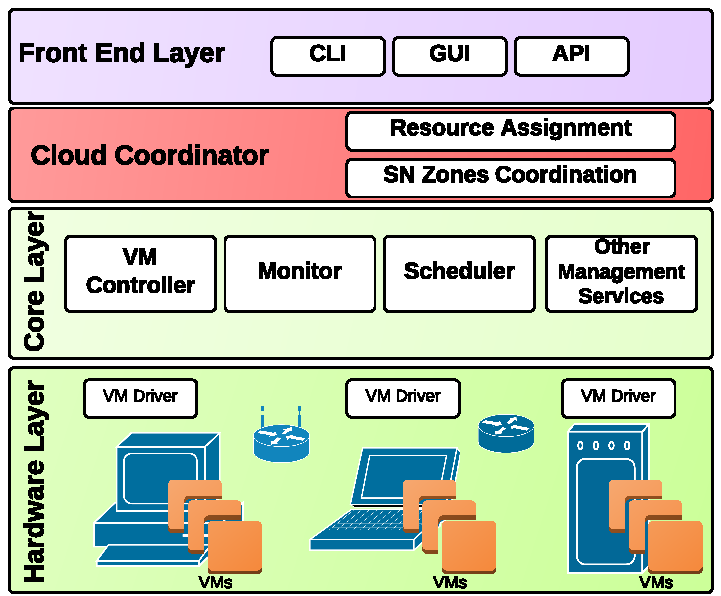
\includegraphics[width=3.5in, keepaspectratio]{vmm-architecture-generic}
%	\caption{Architecture of cloud management system}
%	\label{fig:overview-vmm-hierarchy}
%\end{figure}
%
%\subsubsection{Hardware Layer}
%This consists of the physical infrastructure that is needed to run a cloud system. 
%The hardware in the community networks mostly consists of ONs and SNs and the communication infrastructure, along with any attached computation, storage and other resources.
%
%\subsubsection{Core Layer}
%The core layer consists of components that are responsible for creation, allocation, scheduling, monitoring and management of VMs on the nodes. 
%This can include the following components, some of which are shown in Figure~\ref{fig:overview-vmm-hierarchy}.
%
%\begin{itemize}
%    \item Virtual Machines Controller
%    \item Virtual Machines Scheduler
%    \item Virtual Machines Monitor
%    \item Hosts Manager
%    \item Virtual Network Manager
%    \item Virtual Machines Image Data Store
%\end{itemize}
%
%The functionality of the core layer is already provided by tools like OpenStack and others.
%Community cloud manager can, therefore, make use of these existing tools and extend their functionality to suit the needs of the community network.   
%
%
% %%%%%%%%%%%%%%%%%%%%%%%%%%%%%%%%%%%%%%%%
%\subsubsection{Cloud Coordinator}
%The cloud coordinator is responsible for the federation of the cloud resources which are independently managed by different SNs.
%The cloud coordinator components in different SNs connect among themselves in a decentralised manner to exchange relevant information about managing the available resources.
%Normally applications running at a local community cloud can only consume resources from the ONs directly managed by that particular SN.
%With the cloud coordinator, the infrastructure service can provide a unified view of the resources contributed by multiple local community clouds.
%Figure~\ref{fig:cloud-coordinator-arch} shows the implemented components of the cloud coordinator in the prototype as described below.
%
%\begin{itemize}
%
%    \item{ON Management:} ONs can register with SN to request and to contribute resources.
%
%    \item{Regulation Mechanism:} When pooling resources from multiple zones, the cloud coordinator applies a regulation mechanism that takes into account resource utilisation and contribution by different nodes to perform resource allocation. 
%
%    \item{SN Interconnectivity:} The design of a community cloud manager follows a decentralised approach, so cloud coordinator relies on gossip-based discovery mechanisms to manage overlay network of the SNs in community cloud.
%    The updated list of adjacent SNs is saved in SN-List database.
%
%    \item{SN Resource Sharing:} When requests from ONs cannot be met from locally available resources, SN can request resources from other SNs in the system.
%
%\end {itemize}
%
%%% FIGURE
%\begin{figure}[tbp]
%	\centering
%	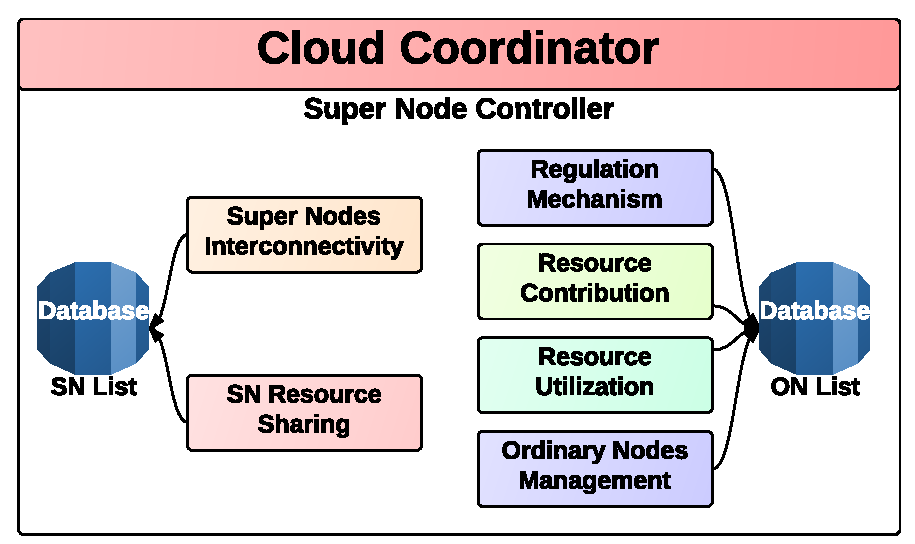
\includegraphics[width=3.5in, keepaspectratio]{vmm-cordinator-arch}
%	\caption{Components of cloud coordinator}
%	\label{fig:cloud-coordinator-arch}
%\end{figure}
%
%
%\subsubsection{Frontend Layer}
%The frontend layer provides the interface to interact with the infrastructure service of the community cloud. 
%This includes modules like command line interface (CLI), graphical user interface (GUI), application programming interface (API), and any other tools that assist with developing cloud application using the infrastructure service.  
%
%
%%%%%%%%%%%%%%%%%%%%%%%%%%%%%%%%%%%%%%%%%
%\subsection{Interaction between Super and Ordinary Nodes}
%
%The overlay network that results from the hierarchical architecture of the community cloud is formed by SNs.
%The difference between SNs and ONs, from the point of view of cloud management, is that SNs support greater functionality for handling VMs. 
%A SN has full installation of the cloud management software and so enables the user to manage VMs executing on ONs.
%In most cases, a SN will be a comparatively stable node, most likely connected to a hub of the wireless mesh network. 
%Each SN is responsible for a set of ONs and manages their metadata in its ON-List database. 
%SNs publish their status and details of local resources to other SNs, e.g. by gossiping, and each SN stores this information in SN-List database.
%ONs, on the other hand, only act as hosts for executing VMs. 
%Most components of cloud management software are not installed on ONs, so the VMs cannot be controlled conveniently from the ONs themselves.
%Each ON registers to a parent SN by providing it with the list of the available resources, and the parent SN is responsible for management of VMs. 
%ONs periodically send a heartbeat message to their parent SN to inform it about their current status.
